\FloatBarrier

\section{COMMUNICATION-SENSING TRADEOFF SYNTHESIS}

Building on the Section II metric-governance contract and the Section IV taxonomy state, Section V operationalizes the standardized reporting-contract and trade-off-synthesis promise introduced in Section I by converting broad study-level evidence into governed, scenario-level quantitative interpretation. It should therefore be read as the review's admissibility-controlled synthesis layer: Section IV determines which records are structurally comparable, and Section V asks what remains quantitatively interpretable once plane and metric-role consistency are enforced.

\subsection{Communication Metrics}
Section V-A works on governed scenario records by default rather than corpus-level study counts. Communication metrics are scoped to reported communication rate ($R$) and link-quality indicators, with strict separation between optical-plane OSNR and electrical-plane SNR/ESNR. This separation is not stylistic; it is required because OSNR and SNR are measured at different receiver-chain stages and are not numerically comparable without an explicit conversion model. The text corpus also supports treating communication outcomes as a primary trade-off axis: across 2,343 extracted snippets (220 papers), communication-centric objectives appear with DIRECT evidence in 167 snippets (124 papers), and explicit trade-off wording appears with DIRECT evidence in 157 snippets (92 papers). Therefore, Table V inventories plane-aware communication coverage, while Fig.~\ref{fig:fig_v_1} later turns the governed subset into role-separated operating views without collapsing measurement planes.

\begin{table}[htbp]
\caption{Governed Communication-Metric Coverage and Plane-Aware Availability}
\label{tab:comm_metrics}
\centering
\setlength{\tabcolsep}{4pt}
\renewcommand{\arraystretch}{1.12}
\begin{tabularx}{\textwidth}{@{}L{2.5cm}Y Y L{2.2cm}Y@{}}
\toprule
\thead{Communication metric} & \thead{Raw scenario coverage} & \thead{Governed usable coverage} & \thead{Governed range /\\median} & \thead{Interpretation note} \\
\midrule
Rate ($R$) & 197/225 records; 194/220 papers & 33 rate-bearing records within 53 governed scenarios & 25 Mbps to 448 Gbps; median 10 Gbps & Supports comparative communication synthesis only with explicit support-size caveats \\
Electrical-plane SNR & 190/225 records; 186/220 papers & 20/53 governed records & 7--22 dB; median 10 dB & The only governed quality indicator that survives filtering across more than one medium slice \\
Optical-plane OSNR & 169/225 records; 166/220 papers & 0/53 governed records & -- & All OSNR-bearing records are blocked by plane-mixing in this release \\
\bottomrule
\end{tabularx}
\end{table}

Before governance filtering, communication reporting appears broad. The trade-off point set contains 225 scenario records from 220 papers, with rate reported in 197/225 records (87.6\%), electrical-plane SNR in 190/225 (84.4\%), and optical-plane OSNR in 169/225 (75.1\%). At paper level, at least one rate value appears in 194/220 papers, at least one SNR value in 186/220 papers, and at least one OSNR value in 166/220 papers. However, raw prevalence should not be confused with synthesis readiness. All 169 OSNR-bearing records co-report SNR and are flagged as plane-mixed, which means that unfiltered counts overstate the amount of quality evidence that can support defensible cross-study comparison.

Applying the Section II governance contract reduces this pool substantially. Of 225 scenario records, 172 (76.4\%) are blocked and 53 (23.6\%) remain usable. The dominant blocker is metric-plane mixing (169 records), followed by $\Delta z$-to-$\Delta r_{\min}$ aliasing flags (19 records); 16 records exhibit both issues. In addition, IM/DD-OSNR inconsistency is present in 98 records, while no SNR-ambiguity flags are observed in this release. At paper level, 169 papers have all scenarios blocked, leaving 51 papers with at least one governed usable scenario. Consequently, Section V-A evidence is intentionally selective: it prioritizes measurement consistency over nominal coverage.

Medium-conditioned rate behavior is interpretable only on the 53 governed records and must be read with explicit sample-size caveats. The usable distribution across normalized medium labels is hybrid (27), cabled fiber (15), wireless FSO (5), generic wireless (2), wireless VLC (1), wireless RF (1), terahertz (1), and other (1). Rate-bearing usable records are concentrated in hybrid (17) and cabled fiber (12). Hybrid rates span 0.025--128 Gbps (median 10 Gbps), while cabled fiber spans 0.04--448 Gbps (median 28.5 Gbps). In contrast, singleton media should be interpreted as anchors rather than distributions: wireless FSO (120 Gbps), wireless VLC (0.125 Gbps), wireless RF (1 Gbps), and terahertz (1 Gbps). Therefore, Table V and Fig.~\ref{fig:fig_v_1} report these slices with sample-size values and avoid modality-wide ranking claims from sparse supports.

Quality-indicator synthesis becomes more constrained after filtering. In the governed subset, electrical-plane SNR remains in 20 records, whereas optical-plane OSNR remains in 0 records. SNR-bearing governed records are primarily hybrid (10) and cabled fiber (8), with smaller contributions from wireless FSO (1) and terahertz (1). Reported SNR ranges are 7--20 dB for hybrid (median 10 dB) and 10--22 dB for cabled fiber (median 10 dB), with single-point values of 13.75 dB (wireless FSO) and 10 dB (terahertz). Because no governance-usable OSNR records survive, this subsection can describe electrical-plane quality patterns but cannot make quantitative optical-plane quality comparisons across media. Table V reports this absence explicitly as an evidence gap rather than hiding it in aggregate summaries.

A communication-resolution coupling view is admissible only inside CRQ-eligible records. The eligible set contains 20 records (all with non-null CRQ values), dominated by hybrid (14), followed by cabled fiber (4), plus one terahertz and one wireless FSO point. This restriction is consistent with the aliasing guardrail: $\Delta z$ is not a surrogate for $\Delta r_{\min}$, and no governed record in this subsection relies on $\Delta z$ substitution. Therefore, CRQ references in V-A are contextual and eligibility-bounded, while full frontier interpretation is deferred to the dedicated trade-off subsection.

Limitations remain material and are stated directly. The contract-violation audit reports 299 MAJOR violations across 169 papers: 261 metric-plane violations and 38 metric-aliasing violations. This imbalance explains why communication evidence appears abundant before filtering but sparse after governance enforcement. Therefore, the V-A conclusions are robust to plane/alias confounding by construction, yet sensitive to current reporting practice in the literature. A practical implication for future corpus growth is straightforward: plane-explicit quality reporting is required to recover optical-plane comparability in cross-medium synthesis.

\begin{quote}
\textbf{Lesson (V-A):} communication evidence in O-ISAC is numerically rich, but only plane-consistent and alias-free subsets support defensible comparative synthesis.
\end{quote}

\subsection{Sensing Metrics}
Section V-B keeps the same governed scenario scope but reorganizes sensing evidence by function rather than by lexical surface form. $\Delta r_{\min}$ represents physical resolution, $\sigma_r$ represents estimator-level accuracy, CRB provides bound-level context, and $\Delta z$ denotes fiber spatial granularity. These roles are not interchangeable, and quantitative comparison is admitted only when role consistency is preserved. Therefore, Table VI summarizes role-separated sensing evidence, while Fig.~\ref{fig:fig_v_1} later preserves separate resolution and accuracy layers instead of a pooled sensing cloud. This framing also aligns with the qualitative record, where trade-off wording is present but unevenly explicit across studies.

\begin{table}[htbp]
\caption{Governed Sensing-Metric Coverage by Functional Role}
\label{tab:sensing_metrics}
\centering
\setlength{\tabcolsep}{4pt}
\renewcommand{\arraystretch}{1.12}
\begin{tabularx}{\textwidth}{@{}L{2.6cm}Y Y L{2.2cm}Y@{}}
\toprule
\thead{Sensing role} & \thead{Raw scenario coverage} & \thead{Governed usable coverage} & \thead{Governed range /\\median} & \thead{Interpretation note} \\
\midrule
Resolution ($\Delta r_{\min}$-eligible) & 173/225 eligible records; 170/220 papers & 20/173 eligible records & 0.0025 m to 15 m; median 0.0397 m & Physical resolution is retained only on the role-consistent governed subset \\
Accuracy ($\sigma_r$) & 186/225 records; 183/220 papers & 16/186 records & 0.001 m to 1000 m; median 0.0575 m & Estimator-level accuracy remains distinct from resolution and is not pooled with $\Delta r_{\min}$ \\
CRB & 148/225 records; 145/220 papers & 0/148 records & -- & Bound-level reporting remains contextual only after governance filtering \\
Fiber spatial granularity ($\Delta z$) & 161/225 records; 158/220 papers & 0/161 records & -- & $\Delta z$ is retained as fiber-specific context and is never substituted for $\Delta r_{\min}$ \\
\bottomrule
\end{tabularx}
\end{table}

Before governance filtering, sensing coverage appears broad at both scenario and paper levels. Across 225 scenario points, $\Delta r_{\min}$ is reported in 195 records (86.7\%), with 173 records (76.9\%) marked $\Delta r_{\min}$-eligible; $\sigma_r$ appears in 186 records (82.7\%); CRB appears in 148 records (65.8\%); and $\Delta z$ appears in 161 records (71.6\%). Paper-level coverage remains similarly high: 192/220 papers report $\Delta r_{\min}$, 170/220 include at least one $\Delta r_{\min}$-eligible scenario, 183/220 report $\sigma_r$, 145/220 report CRB, and 158/220 report $\Delta z$, although only 27/220 contain $\Delta z$-eligible contexts under the contract. Consequently, extraction-level richness is substantial, but direct comparability is still contingent on governance compliance.

After governance filtering, the synthesis-ready subset contracts sharply. Only 53/225 scenarios (23.6\%) remain usable overall, while 172/225 (76.4\%) are blocked. At role level, only 20/173 $\Delta r_{\min}$-eligible records survive (11.6\%), and only 16/186 $\sigma_r$ records survive (8.6\%). In contrast, both CRB and $\Delta z$ drop to zero usable records in the retained subset (0/148 and 0/161, respectively). The exclusion pattern is highly structured rather than random: among blocked $\Delta r_{\min}$-eligible records, 151/153 are plane-mixed; among blocked $\sigma_r$ records, 169/170 are plane-mixed; among blocked CRB records, 147/148 are plane-mixed. Therefore, Table VI distinguishes reported coverage from governance-usable coverage, because raw prevalence alone overstates comparative readiness.

Medium-conditioned resolution behavior can be interpreted only within the 53 governed records and must be read with explicit sample-size caveats. $\Delta r_{\min}$-eligible usable records are concentrated in hybrid (14) and cabled fiber (4), with single records in wireless FSO (1) and terahertz (1). Across all usable $\Delta r_{\min}$-eligible points, $\Delta r_{\min}$ spans 0.0025--15 m, with a median of 0.0397 m. However, within-medium profiles differ materially: hybrid spans 0.0025--10 m (median 0.0191 m), whereas cabled fiber spans 0.01--15 m (median 5.5 m). In contrast, wireless FSO and terahertz each contribute one value (0.0025 m and 0.1 m), so they should be interpreted as anchors rather than distributions. Consequently, cross-medium ranking should be avoided unless the claim is explicitly conditioned on support size and task context.

Estimator-level accuracy shows a distinct governed profile and should not be conflated with resolution. Only 16 usable records report $\sigma_r$: hybrid (8), cabled fiber (7), and terahertz (1). Overall, $\sigma_r$ spans 0.001--1000 m with a median of 0.0575 m, but this range is strongly medium- and scenario-conditioned. Hybrid values cluster between 0.001 and 0.1 m (median 0.01 m), whereas cabled fiber spans 0.001--1000 m (median 1 m), indicating heterogeneous operating assumptions and estimator regimes. Moreover, only 13 usable records contain both $\Delta r_{\min}$-eligible and $\sigma_r$ values. That asymmetry is exactly why Fig.~\ref{fig:fig_v_1} keeps a separate accuracy panel instead of collapsing resolution and accuracy onto one sensing axis.

CRB and $\Delta z$ should be treated as constrained context in this subsection. Although CRB is reported in 148 raw records, none remains governance-usable after filtering, so CRB cannot replace measured $\sigma_r$ in quantitative comparison. Likewise, $\Delta z$ appears in 161 raw records but has zero usable entries in the retained subset and remains explicitly non-substitutable for $\Delta r_{\min}$. This is consistent with the aliasing guardrail: 19 records are flagged for $\Delta z$-to-$\Delta r_{\min}$ aliasing, and any ranging-style inference from $\Delta z$ would violate the contract. In contrast, CRQ-linked comments remain admissible only within CRQ-eligible records (20 records, all within the usable subset).

Measurement-plane discipline further constrains sensing-quality interpretation. In the usable subset, OSNR remains absent (0 records for both $\Delta r_{\min}$-eligible and $\sigma_r$ subsets), while electrical-plane SNR remains available in 12/20 $\Delta r_{\min}$-eligible records and 14/16 $\sigma_r$ records. Therefore, V-B can support limited electrical-plane-conditioned sensing remarks, but cannot support optical-plane-conditioned sensing comparisons across media. This absence is itself informative for Table VI: governed sensing evidence currently depends on post-detection quality reporting rather than optical-plane quality reporting.

The qualitative evidence is consistent with this quantitative contraction. Trade-off mention extraction reports 187 mentions (26 DIRECT, 60 INDIRECT, 101 NONE). DIRECT mentions concentrate in capacity-resolution quotient (11) and resource-allocation trade-off (7), while DIRECT rate-resolution trade-off mentions are sparse (2) and DIRECT Fisher-information-constraint mentions remain limited (4). Therefore, explicit sensing-role articulation exists, but strong synthesis-ready articulation is still a minority pattern relative to total mention volume.

Limitations are material and remain explicit. The governance audit records 299 MAJOR violations across 169 papers, including 261 metric-plane violations and 38 metric-aliasing violations. This profile explains why reported sensing coverage is high before filtering but sharply reduced after governance enforcement. Consequently, V-B conclusions are intentionally conservative: they preserve role-consistent and plane-consistent comparability at the expense of sample size.

\begin{quote}
\textbf{Lesson (V-B):} sensing evidence in O-ISAC is abundant in raw reporting, but defensible cross-medium synthesis requires strict role separation and governance filtering.
\end{quote}

\subsection{Sensing-Communication Trade-off}
Section V-C is the synthesis core of the section: it converts the governed metric subsets into operating-cloud and frontier-style views without relaxing the Section II contract. Rate-versus-resolution is interpreted through rate and $\Delta r_{\min}$, whereas rate-versus-accuracy is interpreted through rate and $\sigma_r$; CRB remains bound-level context, and $\Delta z$ is never treated as a surrogate for $\Delta r_{\min}$. Accordingly, Fig.~\ref{fig:fig_v_1} shows the governed operating clouds at the role-separated level, Fig.~\ref{fig:fig_v_2} zooms into the CRQ-valid frontier subset, and Table VII carries the comparative slice summary with explicit support sizes.

\begin{figure}[htbp]
    \centering
    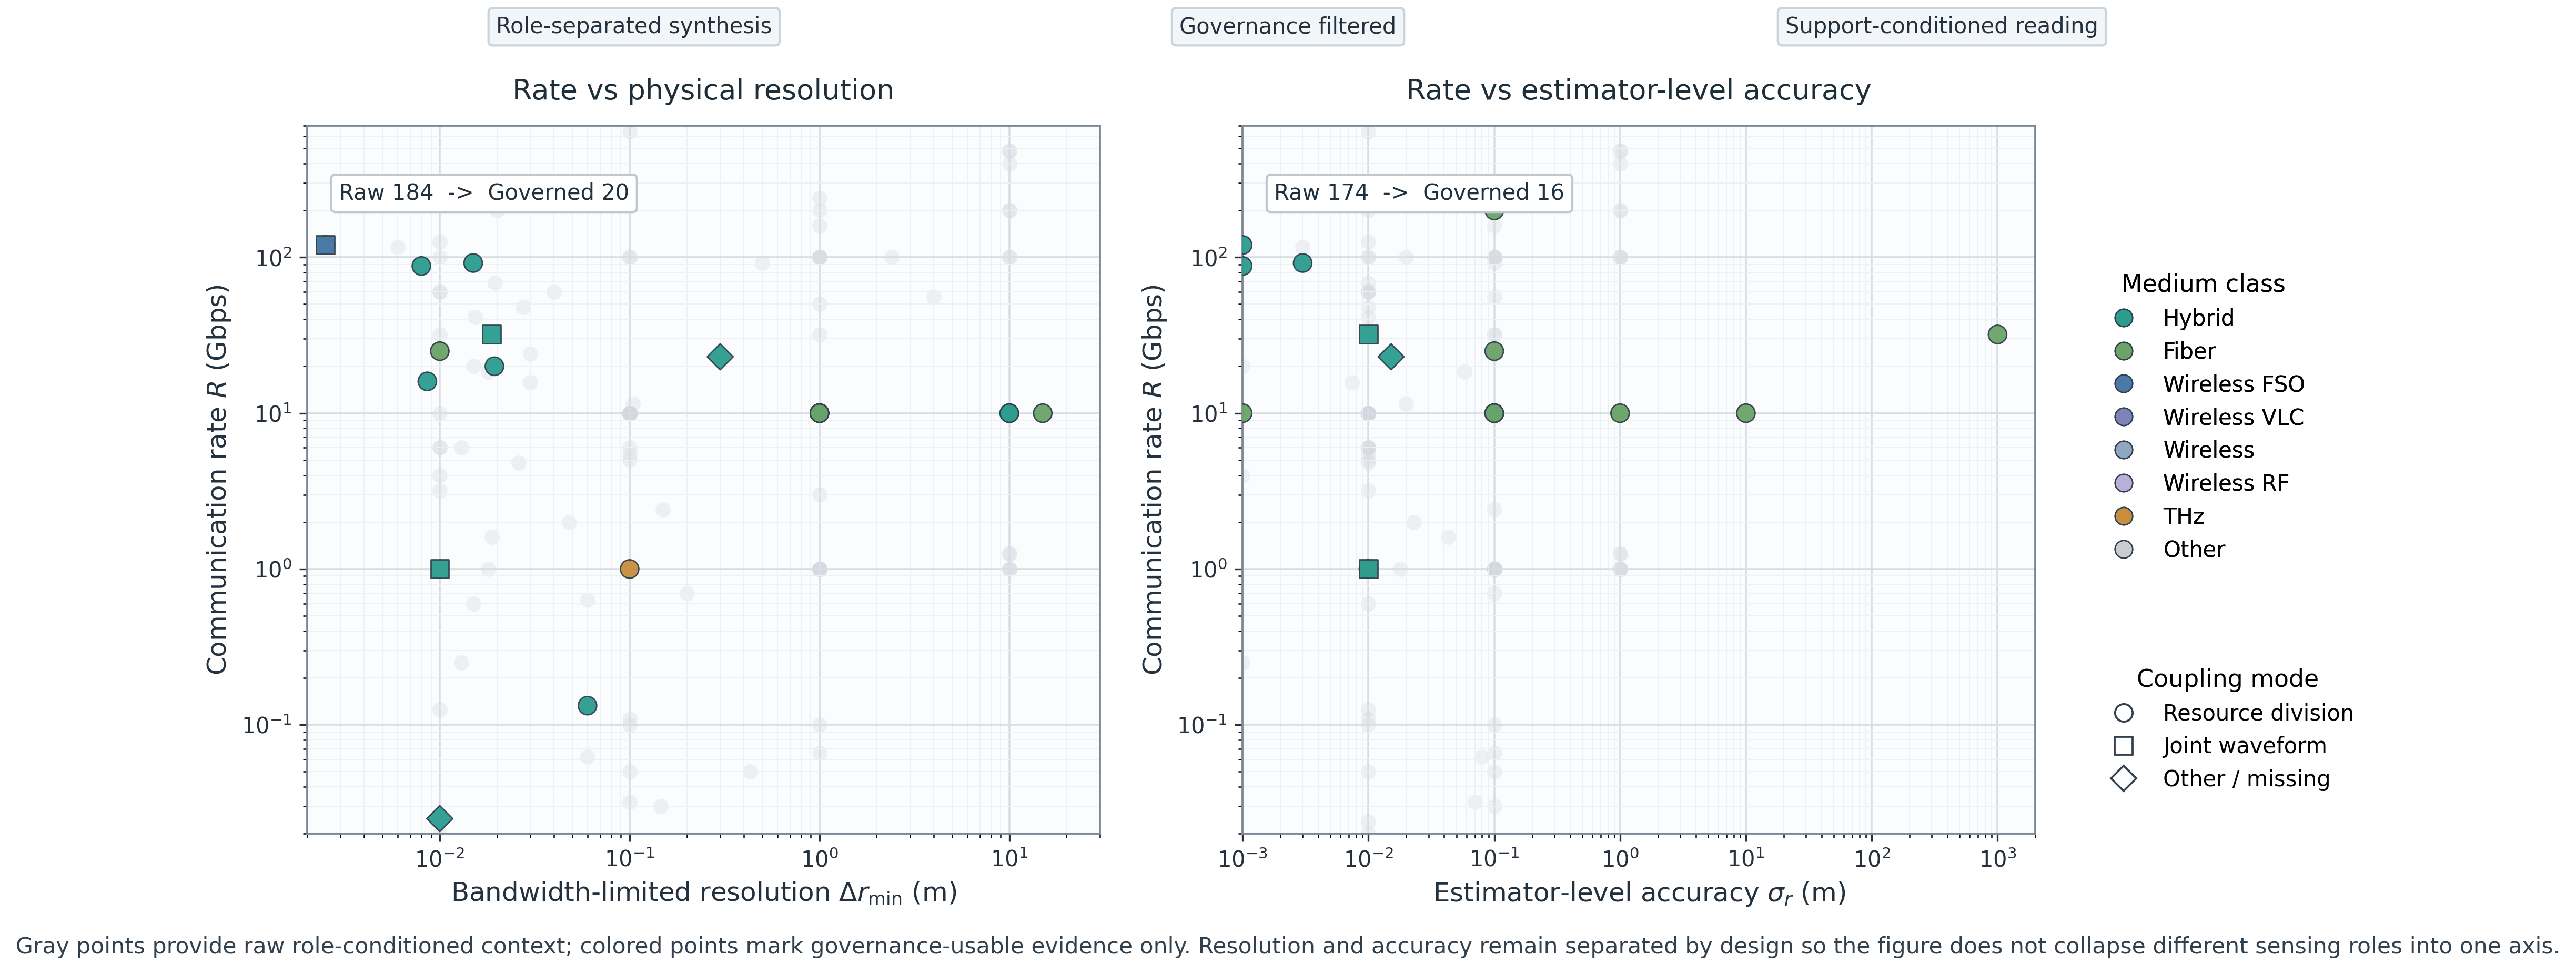
\includegraphics[width=\linewidth]{figures/fig_v_1.png}
    \caption{Reader-facing governed operating clouds for Section V. The left panel shows rate-versus-$\Delta r_{\min}$ evidence after admissibility filtering, whereas the right panel shows rate-versus-$\sigma_r$ evidence under the same governed policy. Gray points denote role-conditioned raw context, colored points denote governance-usable records, and the separated panels make explicit that physical resolution and estimator-level accuracy are synthesized as different sensing roles rather than pooled into one axis.}
    \label{fig:fig_v_1}
\end{figure}

The full trade-off table contains 225 scenario points from 220 papers, but Fig.~\ref{fig:fig_v_1} deliberately does not display that entire set as one comparable cloud. Instead, its gray backgrounds act as role-conditioned raw contexts for the resolution-bearing and accuracy-bearing records, while governance filtering retains only 20 admissible rate-plus-$\Delta r_{\min}$ points and 16 admissible rate-plus-$\sigma_r$ points. At paper level, only 51 papers contribute at least one governed usable point. This contraction is not a peripheral cleanup; it determines the admissible evidence for trade-off inference. Consequently, V-C addresses both the shape of the governed region and the magnitude of evidence loss relative to the nominal cloud. In contrast, treating the raw cloud as fully comparable would overstate the maturity of cross-study trade-off evidence.

Trade-off dimensions are present in labels, but not always in governed metric content. In the raw set, 212 points carry rate-versus-RMSE labeling and 35 carry rate-versus-range-resolution labeling; in the usable subset, these counts become 47 and 5, respectively. However, only 14 of the 47 usable rate-versus-RMSE-labeled points actually report $\sigma_r$, and none of the 5 usable rate-versus-range-resolution-labeled points is $\Delta r_{\min}$-eligible. Therefore, dimensional interpretation in V-C is grounded in governed metric availability rather than label strings alone. Consequently, labels are treated as narrative cues, while eligibility-filtered fields define the quantitative core.

Coupling-mode coverage exhibits a similar asymmetry. Across all 225 points, \texttt{resource\_division} appears in 180 points and \texttt{joint\_waveform} in 41 points, with 4 points carrying missing or non-standard coupling labels. In the 53 governed points, \texttt{resource\_division} remains dominant (38), \texttt{joint\_waveform} remains secondary (13), and 2 points remain unlabeled. Therefore, coupling comparisons are informative but incomplete, and Table VII preserves an explicit unlabeled category for auditability rather than forcing every point into a binary allocation.

The governed operating region can still be summarized numerically with clear caveats. Within the usable subset, rate is reported in 33 points, spanning 25 Mbps to 448 Gbps with a median of 10 Gbps. $\Delta r_{\min}$-eligible values appear in 20 points, spanning 0.0025--15 m (median 0.0397 m), while $\sigma_r$ appears in 16 points, spanning 0.001--1000 m (median 0.0575 m). Overlap remains limited: 20 points support rate-plus-$\Delta r_{\min}$ interpretation, 16 support rate-plus-$\sigma_r$ interpretation, and only 13 support the full triplet (rate, $\Delta r_{\min}$, $\sigma_r$). Therefore, Fig.~\ref{fig:fig_v_1} presents separate resolution-coupled and accuracy-coupled layers rather than a pooled sensing axis.

CRQ partitioning makes admissibility compression explicit. The point taxonomy is 225 total points, 170 CRQ-candidate points, 20 CRQ-valid points, and 2 Pareto points; these totals are consistent with the Section V summary table. The transition from candidate to valid points (170 to 20) is substantial, and frontier evidence is sparse by design (2 points). Fig.~\ref{fig:fig_v_2} therefore visualizes only the last two layers of that compression rather than the full raw cloud. Within governed records, all CRQ candidates are valid (20/20), indicating that most admissibility selection occurs before frontier extraction. Consequently, CRQ claims in V-C are restricted to the 20 valid records and should not be extrapolated to the full raw cloud.

Within the CRQ-valid set, medium-conditioned heterogeneity remains visible but support is uneven. The 20 valid points are distributed across hybrid (14), cabled fiber (4), terahertz (1), and wireless FSO (1). CRQ spans $6.67 \times 10^8$ to $4.8 \times 10^{13}$ bps/m, with a median of $4.33 \times 10^{10}$ bps/m. Hybrid has the strongest support and a median of $8.83 \times 10^{10}$ bps/m, while cabled fiber has a lower median of $5.5 \times 10^9$ bps/m. However, terahertz and wireless FSO remain single-point anchors. Therefore, cross-medium interpretation should be coverage-weighted and explicitly non-ranking when support collapses to singleton slices.

Pareto interpretation requires an additional caution layer. The Pareto file contains 2 points from 2 papers: one hybrid and one wireless FSO. Both are rate-versus-RMSE points with CRQ value $4.8 \times 10^{13}$ bps/m, and coupling modes split one-to-one between \texttt{resource\_division} and \texttt{joint\_waveform}. Because this frontier is minimal, Fig.~\ref{fig:fig_v_2} should be interpreted as an illustrative boundary snapshot rather than a stable envelope of the O-ISAC design space. Consequently, V-C uses Pareto points as exemplar operating points, not as a basis for modality-wide conclusions.

\begin{figure}[htbp]
    \centering
    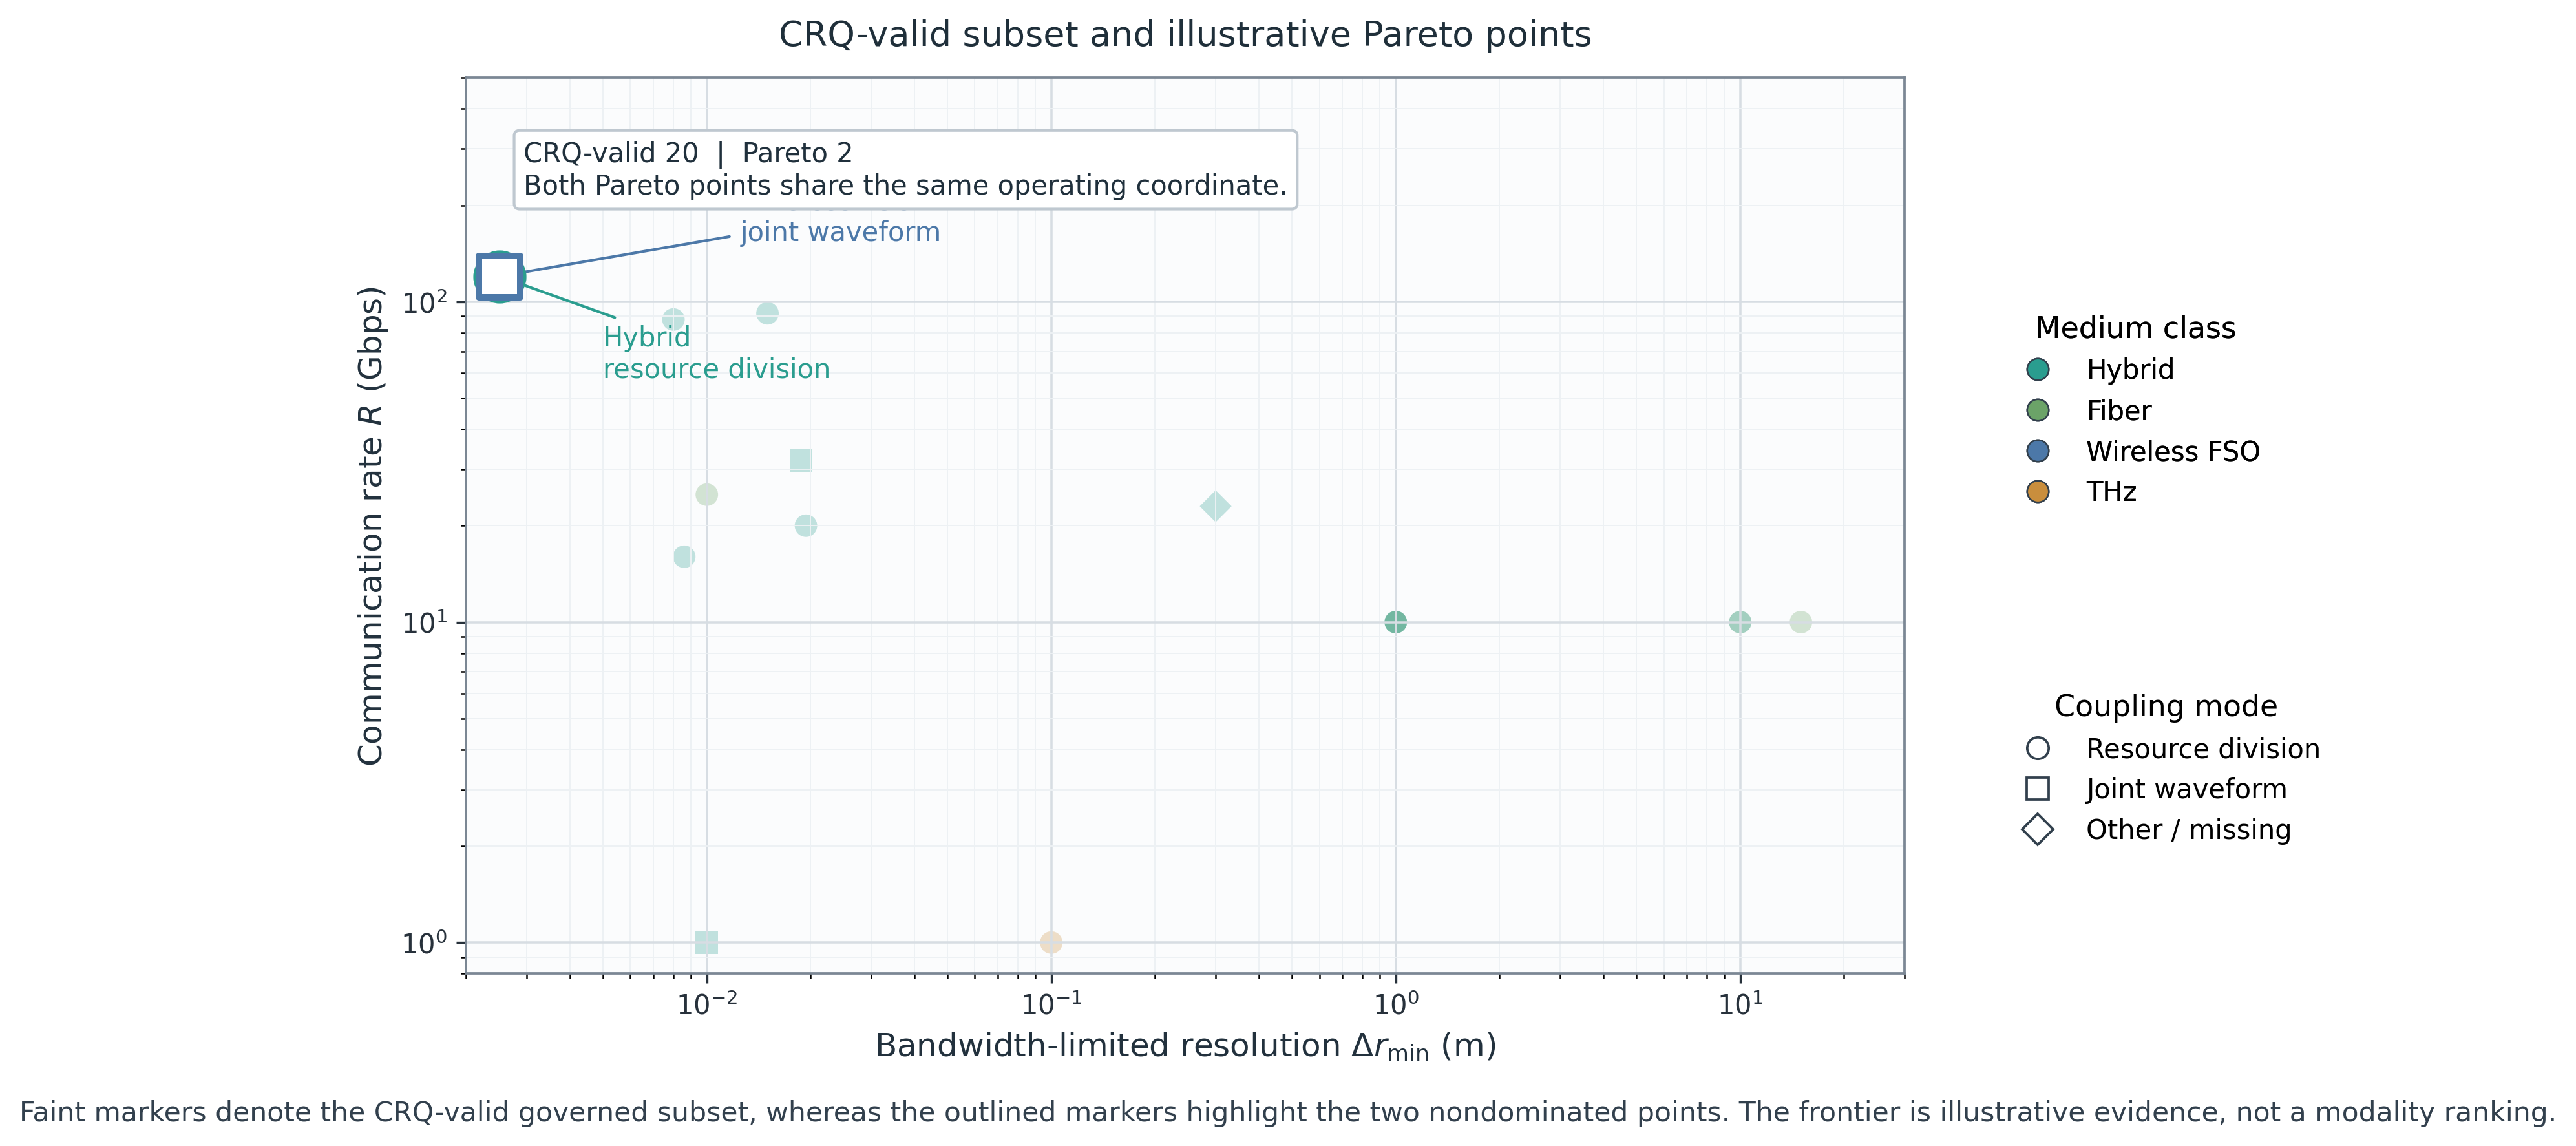
\includegraphics[width=\linewidth]{figures/fig_v_2.png}
    \caption{Reader-facing sparse frontier view for the CRQ-valid subset of Section V. Faint markers denote the 20 governance-usable CRQ-valid points, whereas the enlarged outlined markers denote the 2 nondominated Pareto points. The figure is therefore a zoomed-in frontier illustration rather than a visualization of the full raw trade-off cloud, and it must be read as bounded evidence rather than as a stable modality ranking.}
    \label{fig:fig_v_2}
\end{figure}

Measurement-plane constraints remain active throughout this subsection. In the governed subset, 20 points retain electrical-plane SNR while 0 retain optical-plane OSNR; in the CRQ-valid subset, 12 retain SNR and 0 retain OSNR. Therefore, the trade-off synthesis can condition selected claims on electrical-plane quality but cannot establish optical-plane-conditioned frontier trends. This caveat should remain explicit in Table VII notes and figure captions to avoid implicit cross-plane equivalence.

Qualitative trade-off language supports this conservative interpretation while confirming articulation gaps. Trade-off mention extraction reports 187 mentions across 60 papers: 26 DIRECT, 60 INDIRECT, and 101 NONE. DIRECT mentions are concentrated in capacity-resolution quotient (11) and resource-allocation trade-off (7), with smaller counts for Fisher-information constraints (4), Pareto optimality (2), and rate-resolution trade-off (2). Therefore, explicit trade-off reasoning exists, but it is still a minority pattern relative to total mention volume.

Limitations remain material for V-C. The governance audit reports 299 MAJOR violations across 169 papers, including 261 metric-plane violations and 38 metric-aliasing violations. These violations account for much of the candidate-to-valid compression and the sparse Pareto set. Consequently, V-C conclusions are intentionally conservative: they prioritize role-consistent, plane-consistent, and traceable synthesis over broader but weakly governed aggregation.

\begin{quote}
\textbf{Lesson (V-C):} sensing-communication trade-off evidence is abundant in raw extraction, but defensible operating-region and frontier claims emerge only after strict eligibility partitioning and explicit support-size caveats.
\end{quote}

\subsection{Comparative Analysis: Fiber vs Wireless}
Section V-D keeps the same governed scenario scope but changes the question from ``what is available?'' to ``what can be compared responsibly?''. The comparison protocol has three steps. First, candidate points are filtered by the Section II governance contract (plane separation, metric-role separation, and alias controls). Second, medium labels are kept exactly as normalized in Section IV (\texttt{cabled\_fibre}, \texttt{wireless\_*}, \texttt{hybrid}, and residual classes). Third, comparative claims are restricted to sample-supported slices and reported with explicit coverage caveats. Therefore, Table VII is the primary comparative anchor, and this subsection is framed as evidence-weighted comparison rather than ranking.

\begin{table}[htbp]
\caption{Governed Fiber, Wireless, and Hybrid Slices}
\label{tab:comparative_slices}
\centering
\setlength{\tabcolsep}{4pt}
\renewcommand{\arraystretch}{1.08}
\begin{tabularx}{\textwidth}{L{2.3cm} C{1.6cm} Y Y Y Y Y}
\toprule
Comparative slice & Governed points\\(papers) & Median rate & Median $\Delta r_{\min}$ & Median $\sigma_r$ & Median CRQ\\(eligible only) & Coupling composition \\
\midrule
Fiber (cabled fiber slice) & 15 (13) & 28.5 Gbps (\texttt{n\_rate=12}) & 5.5 m (\texttt{n=4}) & 0.1 m (\texttt{n=7}) & $5.50 \times 10^9$ bps/m (\texttt{n=4}) & \texttt{resource\_division} 13; \texttt{joint\_waveform} 2 \\
Wireless (pooled wireless slice) & 9 (9) & 1 Gbps (\texttt{n\_rate=3}) & 0.0025 m (\texttt{n=1}) & -- & $4.80 \times 10^{13}$ bps/m (\texttt{n=1}) & \texttt{resource\_division} 5; \texttt{joint\_waveform} 4 \\
Hybrid bridge slice & 27 (27) & 10 Gbps (\texttt{n\_rate=17}) & 0.019075 m (\texttt{n=14}) & 0.01 m (\texttt{n=8}) & $8.83 \times 10^{10}$ bps/m (\texttt{n=14}) & \texttt{resource\_division} 19; \texttt{joint\_waveform} 6; unlabeled 2 \\
\bottomrule
\end{tabularx}
\end{table}

The contraction from raw to governed evidence is substantial and directly shapes what can be compared. The raw trade-off set contains 225 scenario points across 12 medium labels, dominated by hybrid (117) and cabled fiber (47), followed by wireless VLC (27), wireless FSO (19), generic wireless (6), and a long tail of low-support classes. Governance filtering blocks 172 points (76.4\%) and retains 53 points (23.6\%). The governed medium mix then becomes hybrid (27), cabled fiber (15), wireless FSO (5), generic wireless (2), wireless RF (1), wireless VLC (1), terahertz (1), and other (1). Consequently, V-D should be interpreted as a constrained synthesis over a reduced admissible set, not as a direct mirror of raw-corpus prevalence.

For the explicit fiber-versus-wireless contrast, the fiber slice uses the normalized cabled-fiber label, whereas the wireless slice pools the normalized \texttt{wireless\_*} labels together with generic wireless. Hybrid remains a bridge class rather than being forced into either endpoint. In the governed set, fiber contributes 15 points from 13 papers, wireless contributes 9 points from 9 papers, and hybrid contributes 27 points from 27 papers. Metric completeness is asymmetric: fiber contributes 12 rate values, 4 $\Delta r_{\min}$ values, and 7 $\sigma_r$ values; wireless contributes 3 rate values, 1 $\Delta r_{\min}$ value, and 0 $\sigma_r$ values; hybrid contributes 17 rate values, 14 $\Delta r_{\min}$ values, and 8 $\sigma_r$ values. Therefore, hybrid remains central for transferability analysis, but endpoint comparison must still be reported without collapsing hybrid into fiber or wireless.

Rate-side medians in governed slices indicate different operating emphases but do not support universal superiority claims. Fiber shows a median rate of 28.5 Gbps (\texttt{n\_rate=12}), wireless shows 1 Gbps (\texttt{n\_rate=3}), and hybrid shows 10 Gbps (\texttt{n\_rate=17}). However, the wireless median is structurally unstable because it comes from a sparse, heterogeneous mix that includes one high-value wireless FSO point and lower-rate entries from other wireless labels. Therefore, Table VII reports median rate together with support counts so that apparent ordering is interpreted as support-weighted evidence.

Sensing-side comparison is more constrained by missingness. In governed slices, fiber has median $\Delta r_{\min}$ of 5.5 m (\texttt{n=4}) and median $\sigma_r$ of 0.1 m (\texttt{n=7}). Wireless has only one $\Delta r_{\min}$ value (0.0025 m) and no governed $\sigma_r$ value. Hybrid has median $\Delta r_{\min}$ of 0.019075 m (\texttt{n=14}) and median $\sigma_r$ of 0.01 m (\texttt{n=8}). Consequently, a limited rate-versus-resolution contrast can be stated between fiber and wireless, but a balanced rate-versus-accuracy contrast cannot be established for this release. In contrast, hybrid supports a dual-metric interpretation because both resolution and accuracy are represented.

CRQ-conditioned comparison should be read through the strict 20-point eligible subset summarized in the modality-slice file. In that subset, hybrid contributes 14 points (median CRQ $8.83 \times 10^{10}$ bps/m), cabled fiber contributes 4 points (median CRQ $5.50 \times 10^9$ bps/m), wireless FSO contributes 1 point ($4.80 \times 10^{13}$ bps/m), and terahertz contributes 1 point ($1.00 \times 10^{10}$ bps/m). This normalization is useful for high-selectivity comparison, but it is intentionally sparse and does not represent the full governed cloud. Therefore, Table VII keeps governed medium slices as the primary comparative artifact and retains CRQ only as a bounded contextual column rather than as a frontier-summary substitute.

Coupling composition adds an additional interpretation layer. Fiber governed points are mostly resource-division (13/15), with a smaller joint-waveform tail (2/15). Wireless points are split more evenly between resource-division (5/9) and joint-waveform (4/9). Hybrid is also resource-division-led (19/27), with joint-waveform support (6/27) and an unlabeled remainder (2/27). Therefore, observed medium-level differences in medians should be read jointly with coupling composition, because allocation strategy and medium are entangled in the reported operating points.

Measurement-plane constraints remain active in this subsection and limit quality-conditioned comparison. In the governed slices, optical-plane OSNR has zero usable entries for fiber, wireless, and hybrid, whereas electrical-plane SNR remains available for fiber (8 points), hybrid (10 points), and one wireless anchor. Consequently, V-D can support limited electrical-plane-conditioned remarks for fiber and hybrid, plus a single wireless reference point, but cannot establish optical-plane-conditioned fiber-versus-wireless trends.

Limitations are explicit and materially relevant for comparative claims. The governance audit reports 299 MAJOR violations across 169 papers, including 261 metric-plane violations and 38 metric-aliasing violations. At paper level, 169/220 papers have all scenarios blocked, leaving 51 papers with at least one governed usable scenario and only 20 papers with CRQ-eligible evidence. Therefore, V-D conclusions are deliberately conservative: they preserve defensible comparison where support exists and mark sparse slices as non-ranking evidence.

\begin{quote}
\textbf{Lesson (V-D):} fiber-versus-wireless comparison in O-ISAC is defensible only under governance filtering, explicit support-size reporting, and explicit treatment of hybrid as a bridge class rather than an endpoint.
\end{quote}

\subsection*{Section V closeout synthesis}
Pareto interpretation in Section V remains bounded by three nested evidence layers: the raw trade-off cloud (225 points), the governed cloud (53 points), and the CRQ-valid subset (20 points) from which only 2 Pareto points are selected. Consequently, Fig.~\ref{fig:fig_v_2} is interpreted as a governance-conditioned frontier view rather than as a direct projection of the raw operating landscape. This compression is analytically central, not cosmetic: candidate abundance does not translate into frontier-level comparability unless plane, role, and eligibility constraints are simultaneously satisfied.

The frontier is also highly selective in composition. Within the CRQ-valid subset, hybrid contributes 14 points, cabled fiber 4, terahertz 1, and wireless FSO 1; however, the Pareto set itself contains only one hybrid point and one wireless FSO point. Therefore, the absence of fiber and terahertz points from the frontier cannot be interpreted as inferiority. It only indicates that current nondominated evidence is sparse and unevenly distributed across media. The same caution applies to coupling mode: the valid set is resource-division-led (15 points versus 3 joint-waveform points, plus 2 unlabeled points), yet the frontier splits one-to-one between \texttt{resource\_division} and \texttt{joint\_waveform}. Accordingly, Section V supports conditional design interpretation, not stable medium-wide or coupling-wide ranking.

Metric-role and measurement-plane constraints remain active at this closing stage. All CRQ-valid points are $\Delta r_{\min}$-eligible, but only 13/20 also report $\sigma_r$, and only 1 of the 2 Pareto points includes $\sigma_r$. Likewise, OSNR is absent from the governed, valid, and Pareto subsets, while electrical-plane SNR remains available in 20 governed points, 12 valid points, and 1 Pareto point. Therefore, frontier interpretation is stronger for rate-versus-resolution than for rate-versus-accuracy, and it cannot support optical-plane-conditioned frontier claims. Fig.~\ref{fig:fig_v_2} should therefore be captioned as sparse illustrative evidence of admissible extreme operating points under the current reporting contract.

These observations still yield practical guidance. Decision-stage claims should be restricted to CRQ-valid evidence rather than to the full candidate cloud; operating-point discussions should report both $\Delta r_{\min}$ and $\sigma_r$ whenever possible; and medium and coupling context should remain attached to every frontier-style interpretation. This bounded reading is consistent with the qualitative trade-off record, where DIRECT trade-off language remains a minority relative to INDIRECT and NONE labels. It also provides the correct handoff to the next sections: Section VI should discuss enablers as mechanisms that may widen the governed evidence base rather than bypass governance, while Section VIII should treat sparse frontier evidence as a challenge signal rather than as proof of maturity. Limitations remain explicit: the governance audit reports 299 MAJOR violations across 169 papers, including 261 metric-plane violations and 38 metric-aliasing violations. Section V therefore closes on a deliberately conservative conclusion: the field already contains strong governed exemplars, but reliable design generalization still depends on expanding the CRQ-valid, medium-balanced evidence base.

\begin{quote}
\textbf{Lesson (V):} governed trade-off synthesis is already informative for bounded engineering interpretation, but frontier-level generalization remains limited by sparse valid support and uneven reporting discipline.
\end{quote}
